%
% Niniejszy plik stanowi przyk³ad formatowania pracy magisterskiej na
% Wydziale MIM UW.  Szkielet u¿ytych poleceñ mo¿na wykorzystywaæ do
% woli, np. formatujac wlasna prace.
%
% Zawartosc merytoryczna stanowi oryginalnosiagniecie
% naukowosciowe Marcina Wolinskiego.  Wszelkie prawa zastrze¿one.
%
% Copyright (c) 2001 by Marcin Woliñski <M.Wolinski@gust.org.pl>
% Poprawki spowodowane zmianami przepisów - Marcin Szczuka, 1.10.2004
% Poprawki spowodowane zmianami przepisow i ujednolicenie 
% - Seweryn Kar³owicz, 05.05.2006

\documentclass[licencjacka]{pracamgr}

\usepackage{polski}

\usepackage[utf8]{inputenc}

\usepackage{pdfpages}


% Dane licencjanta:

\author	{Imię Nazwisko}

\nralbumu{666999}

\title{Implementacja taktycznej gry fabularnej czasu rzeczywistego}

\tytulang{An implementation of a real-time strategy role-playing game}

\kierunek{Informatyka}

\opiekun{mgra Radosława Bartosiaka\\
  Instytut Informatyki\\
  }

% miesiąc i rok:
\date{Maj 2015}

\dziedzina{11.3 Informatyka}

%Klasyfikacja tematyczna wedlug ACM (informatyka)
\klasyfikacja{D. Software}

\keywords{gra, gra komputerowa, qt, sfml, box2d, taktyczna gra fabularna}

% Tu jest dobre miejsce na Twoje własne makra i środowiska:
% \newtheorem{defi}{Definicja}[section]

% koniec definicji

\begin{document}
\maketitle

%tu idzie streszczenie na strone poczatkowa
\begin{abstract}
  Niniejsza praca opisuje taktyczną grę fabularną stworzoną
  w~ramach przedmiotu Zespołowy Projekt Programistyczny.
  W~szczególności opisane zostało projektowanie silnika,
  mechaniki oraz~interfejsu gry. Praca zawiera również 
  opis osiagniętego rezultatu wraz z~wynikiem przeprowadzonych testów.
\end{abstract}

\tableofcontents
%\listoffigures
%\listoftables

\chapter*{Wprowadzenie}
\addcontentsline{toc}{chapter}{Wprowadzenie}


\chapter{Podstawowe pojęcia}

\chapter{Wstęp}

  \section{Opis projektu}

  \section{Grupa docelowa}
 
  \section{Analiza podobnych gier}
 
  \section{Mechanika}
  
  \section{Fabuła}
  
  \section{Interfejs}

\chapter{Narzędzia i metodologia pracy}

  \section{Użyte wzorce projektowe}

  \section{Użyte narzędzia}

  \section{Playtesty}
  \subsection{Cel}
%   UWAGA ten paragraf prawpodobnie będzie trzeba przeredagować z czasem
  Docelowo, od~momentu rozpoczęcia playtestów, cały cykl deweloperski będzie podyktowany 
  kolejnymi iteracjami: playtesty - -- --- wnioski - produkcja. Wraz z~postępami w projekcie, 
  coraz większy nacisk będzie kładziony na doznania gracza i~zbalansowanie gry. 
  Wstępnie planowane są~3~serie playtestów, pierwsza testująca ogólną mechanikę i~interfejs,
  druga sprawdzająca szczegółowo wszystkie mechanizmy gry, trzecia, końcowa, mająca na celu dopracowanie wersji alfa gry.
  Istotnym elementem każdego playtestu jest uzyskanie informacji zwrotnej od~nowych testerów, nieznających koncepcji gry.
    
    \subsection{Testy mechaniki i interfejsu (Faza I)}
    Pierwsza faza testów została przeprowadzona na surowej wersji gry, 
    z~niepełnym zestawem funkcjonalności i~prototypowymi fragmentami grafiki. 
    Był to ostatni moment na~poważne zmiany mechaniki lub~dodanie nowych funkcji silnika.
      
      \subsubsection{Założenia i cele}
      Ta faza testów została zrealizowana na~podstawie ówczesnej wersji deweloperskiej, 
      bez~robienia specjalnej wersji wyłącznie do~tego celu. Jej głownym zadaniem jest 
      wykazanie błędów w~logice zachowania oraz~sprawdzenie wygody i~intuicyjności interfejsu. 
      Pomniejszym celem jest otrzymanie feedbacku od graczy na temat klimatu gry
      i~ewentualnych funkcjonalności, które poprawiłyby jakość końcowego produktu.
      
      \subsubsection{Forma}
      Testy gry na tym etapie składały się z~dwóch części, samodzielnej 15-20 min gry
      oraz swobodnej rozgrywce z dozwoloną ingerencją koordynatora.
      
      Pierwsza część testu polegała na indywidualnej grze na ówcześnie gotowej planszy.
      Każdy gracz otrzymał wydrukowaną instrukcję gry (zawierającej sterowanie i~wstęp fabularny)
      i~powinien był sam zrozumieć cel i~zasady gry. W~tym czasie, zespół udzielał minimalną liczbę
      podpowiedzi (wyłącznie w przypadku wyraźnych problemów gracza z rozgrywką) i~nie ingerował w~test.
      Zadaniem koordynatorów w~tej części było odnotowywanie reakcji gracza. 
      Po ukończeniu rozgrywki gracz wykorzystując stosowną ankietę przepytywał gracza na temat 
      jego ogólnego odbioru gry i~wcześniejszego doświadczenia z~grami. 
      
      Druga część wyglądała podobnie do~pierwszej, jednak zadaniem gracza było wykazanie 
      jak największej liczby błędów i~nieintuicyjnych mechanizmów gry. 
      Podczas tej części zespół na~bieżąco odpowiadał na pytania uczestników,
      a~także zadawał pytania o~opinie i~uwagi gracza na temat poszczególnych funkcjonalności
      lub~prosił o~wykonanie konkretnych zadań (np. otwarcie okna ekwipunku postaci).

      \subsubsection{Ankiety}
      Każdy koordynator był~wyposażony w~3~formularze:
      \begin{enumerate}
	\item arkusz do~wpisywania obserwacji,
	\item arkusz do~notowania błędów i~problemów,
	\item ankieta z~pytaniami do~testera.
      \end{enumerate}
      Każdy tester otrzymywał instrukcję zawierającą sterowanie i~wstęp fabularny.
      
      \noindent
      Wymienione formularze oraz~instrukcja znajdują się w~dodatkach, na~końcu pracy.
  
%   \section{Edytor treści}

\chapter{Kamienie milowe}

  \section{Podstawowy silnik gry (Wersja~0.1)}
  
  \section{Ukończenie przewidzianych funkcjonalności (Wersja~0.2)}
  
  \section{Gotowy produkt (Wersja~1.0)}

\chapter{Wkład własny w powstały system}

  \section{Jan Darowski}

  \section{Piotr Majcherczyk}

  \section{Rafał Soszyński}

  \section{Tomasz Zakrzewski}

\chapter{Rezultat}

  \section{Zrealizowane funkcjonalności}

  \section{Niezrealizowane funkcjonalności}

  \section{Opinie testerów}

  \section{Podsumowanie autorów}

\appendix

  \chapter{Przykładowe zrzuty ekranu}

  \chapter{Materiały do playtestów}
  Na kolejnych stronach znajdują się ankiety używane podczas playtestów
  oraz~instrukcja gry wręczana testerom.

    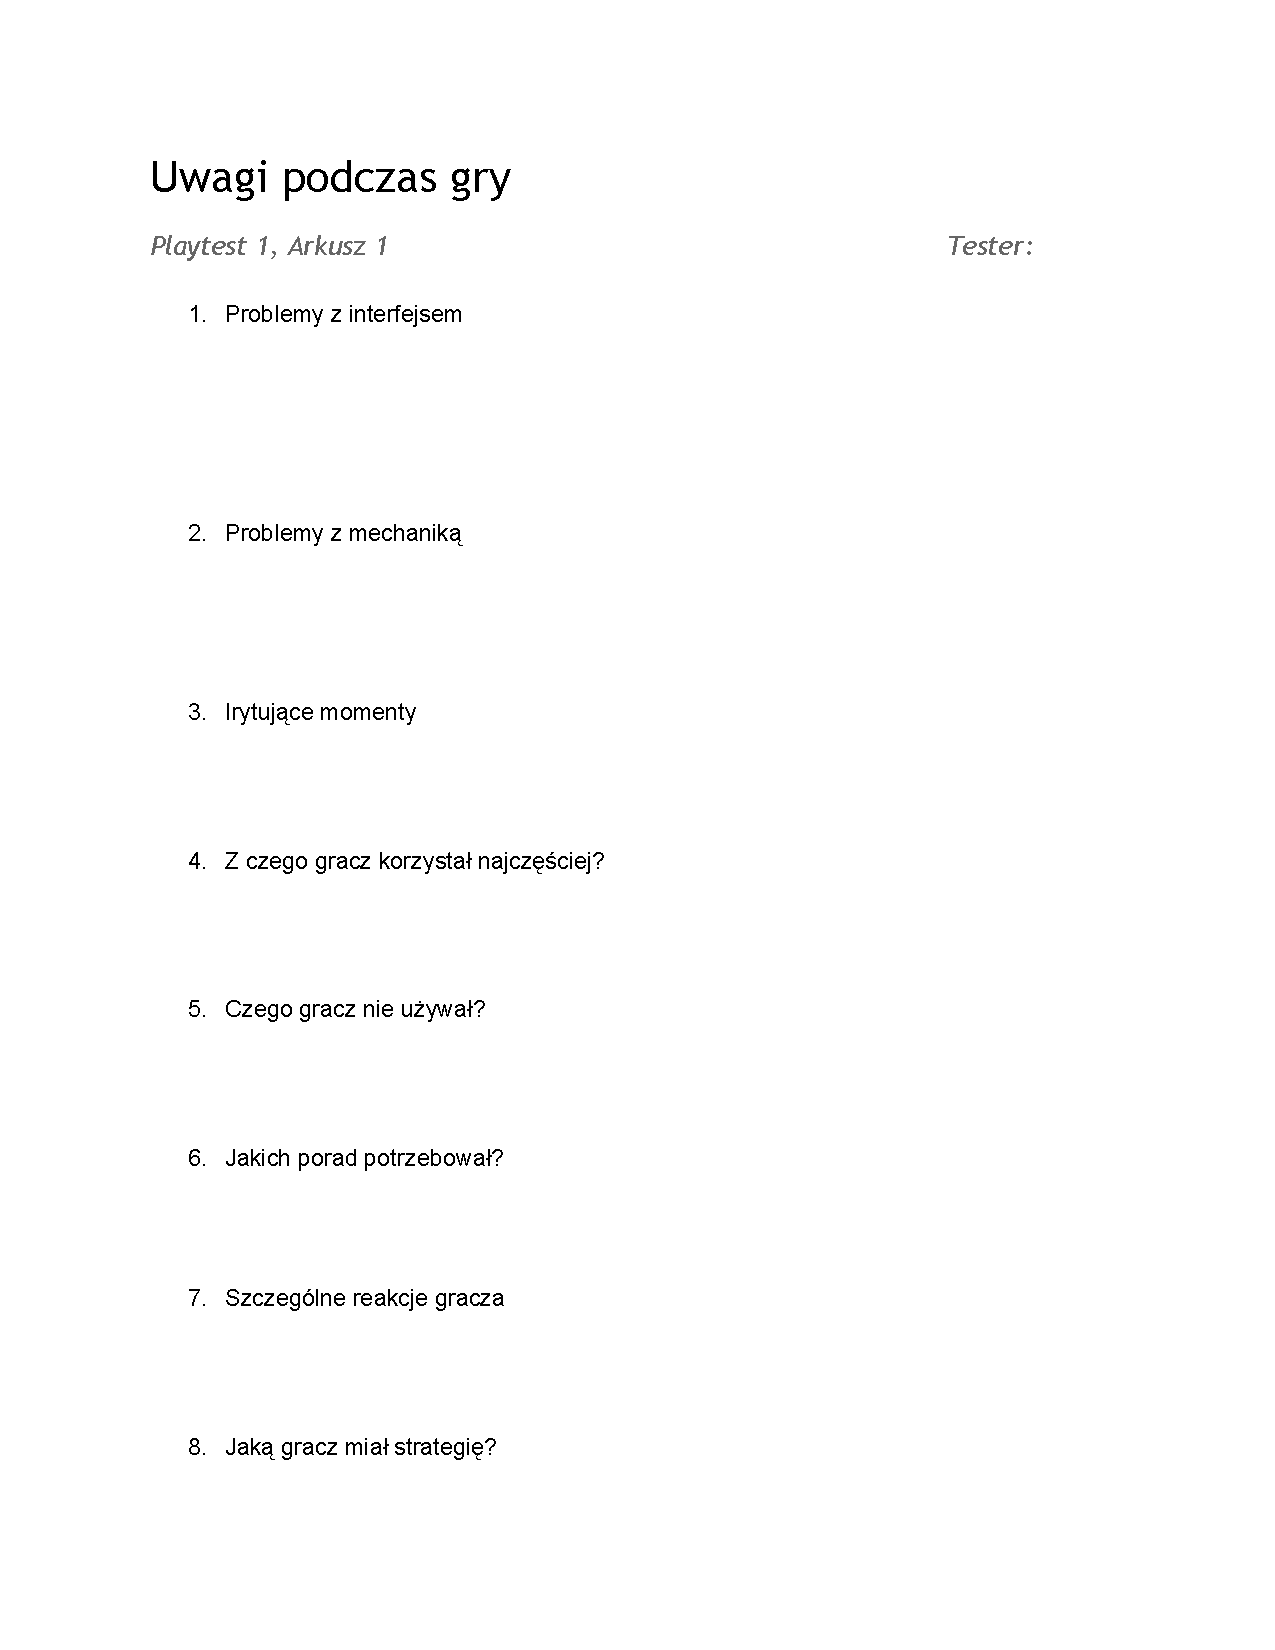
\includepdf[pages={-}]{Formularze-playtesty.pdf}
    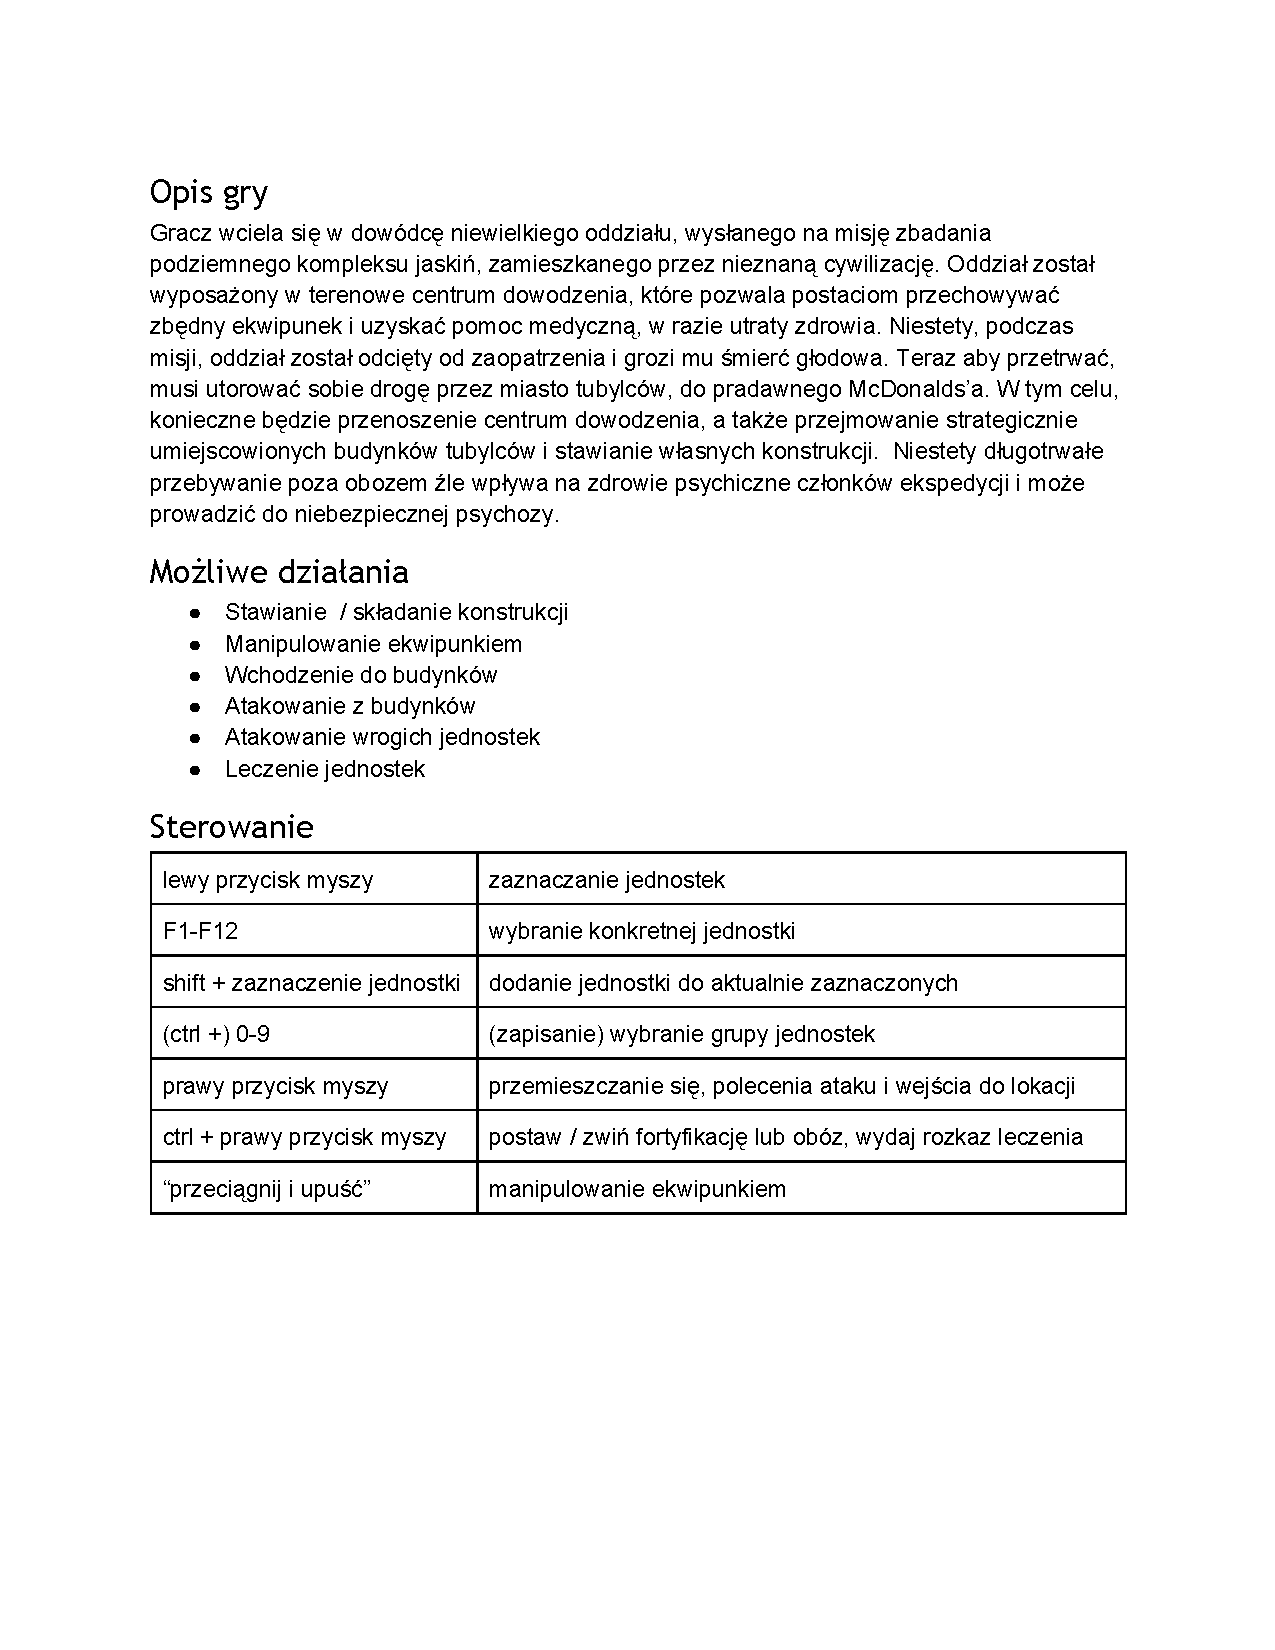
\includepdf[pages={-}]{Instrukcje-do-playtestow.pdf}

  \chapter{Zawarość płyty CD}


\begin{thebibliography}{99}
\addcontentsline{toc}{chapter}{Bibliografia}

  \item{coś tam}

\end{thebibliography}

\end{document}


%%% Local Variables:
%%% mode: latex
%%% TeX-master: t
%%% coding: utf8
%%% End:
